\documentclass[a4paper, 11pt]{article}

%\usepackage[parfill]{parskip}
\usepackage{ragged2e}
\usepackage{graphicx}
\graphicspath{ {images/} }
\usepackage[T1]{fontenc}

\newlength{\drop}
\usepackage{epigraph}
\usepackage{dirtytalk}
\usepackage{wrapfig}
\usepackage{quoting}

%\usepackage[pdftex,active,tightpage]{preview} 
%\setlength\PreviewBorder{2mm} 
\usepackage{gantt}
\renewcommand{\epigraphflush}{center}
\renewcommand{\epigraphwidth}{1\textwidth}

%........................
% Header/Footers
%........................
\usepackage{lastpage}
\usepackage{fancyhdr}

%%%%%%%START%%%%%%%
\begin{document}
  \begin{titlepage}
	\thispagestyle{empty}
    \drop=0.1\textheight
    \centering
    \vspace*{\baselineskip}
    \rule{\textwidth}{1.6pt}\vspace*{-\baselineskip}\vspace*{2pt}
    \rule{\textwidth}{0.4pt}\\[\baselineskip]
    {\Large{MSc Computer Science\\[0.3\baselineskip] }} 	
    {\huge{Project Proposal\\[0.3\baselineskip] }}
	
    \rule{\textwidth}{0.4pt}\vspace*{-\baselineskip}\vspace{3.2pt}
    \rule{\textwidth}{1.6pt}
    \\[\baselineskip]
    \scshape
    {\Large Ubiquitous Consumer Inventory Management System For Waste Prevention\\}
%    Location, date from--to\par
    \vspace*{2\baselineskip}
    %Edited by \\[\baselineskip]
    {\normalsize\emph{Supervisor: }{\large Professor George Roussos\par}}
    {\normalsize\emph{Author: }{\large Keimi Okamoto\par}}
    
    {\itshape 2015}
    \vfill
    {\large BIRKBECK UNIVERSITY OF LONDON\par}
{\footnotesize DEPARTMENT OF COMPUTER SCIENCE \& INFORMATION SYSTEMS}\par
  \end{titlepage}
  
%\maketitle

%........................
% Contents
%.......................
\pagenumbering{roman}
\tableofcontents
\clearpage

%........................
% Epigraph
%........................
\epigraph{\say{Its highest ideal is to make a computer so exciting,
so wonderful, so interesting, that we never want to be
without it. A less-traveled path I call the \say{invisible}; its
highest ideal is to make a computer so imbedded, so fitting,
so natural, that we use it without even thinking about it. I
have also called this notion \say{Ubiquitous Computing}.}}
{\textsc{-Mark Weiser,}\textit{ `Creating the Invisible Interface' 1994}}

\clearpage
%........................
% Abstract
%........................
\abstract{It is estimated that the United Kingdom generates 15 million tonnes of food waste annually.\cite{statistic} This colossal amount of waste has devastating impacts on the economy and society. The majority of this statistic is accountable to the domestic household. Poor inventory keeping and busy lifestyles of the consumer all attribute to waste. This project proposes the exploration of item level identification of groceries using Radio Frequency Identification(RFID) and the positive effects on waste reduction. With the use of RFID, remote access of granular information such as use-by-dates and nutritional information will become ubiquitously available via a Smartphone application. This technology intends to empower the consumer to reduce both food and monetary waste by prevention of over purchasing.}
\newpage



%........................
% Introduction
%........................

\pagestyle{fancy}
\renewcommand{\sectionmark}[1]{\markboth{#1}{}}
\fancyhf{} % sets both header and footer to nothing
\renewcommand{\headrulewidth}{0pt}
\setlength{\footskip}{80pt}
\lhead{}
\chead{}
\rhead{Project Proposal}
\pagenumbering{arabic}
\lfoot{Section \thesection}
\cfoot{\fancyplain{}{\leftmark }} 
\rfoot{\thepage\ of \pageref{LastPage}}

\setcounter{page}{1}
\section{Introduction}

\subsection{Background}
Over production of food is a global issue with waste exceeding two billion tonnes annually\cite{waste}. Such large quantities of waste have severe negative social, environmental and economical impacts. The multifaceted nature of the food supply chain give ample opportunity for waste to occur and inadequate waste prevention methods could cause figures to rise.\cite{FoodWaste} Further more, such complex pipelines pose great difficulties in the accurate quantification of waste generated, meaning that the figures are likely to be higher than reported.\cite{waste} A clear understanding of the chain is necessary to identify the vulnerable components where waste can arise, below is a brief description of each of the three main entities that comprise the chain and their accountability to the statistics.

\paragraph{Producers}At the top is the agriculturalists and farmers who cultivate the plants and livestock. These entities serve as the primary source of supply to the market and respond to orders placed by retailers. Over production is often encouraged by the merchant to compensate for the possibility of an unfruitful harvest or an unexpected and sudden rise in demand.\cite{waste} 

\paragraph{Retailers}The intermediate between producer and consumer are the retailers and vendors. At the time of writing, the most dominant being Supermarkets, namely Sainsbury's, Tesco, Asda and Morrison. Perpetual competition for market share leads to aggressive advertising and competitive pricing wars, with millions of pounds at stake urgency for quantity control becomes a lesser priority. Errors in sales forecasts can result in idle stock needlessly occupying valuable real estate costing millions in rental annually. Waste can even occur on a superficial level where ascetically unpleasing but perfectly consumable food is deemed unworthy of stocking and rejected.\cite{FoodWaste} 

\paragraph{Consumers}At the end of the chain are the consumers that are regularly persuaded to over purchase by enticing bulk buying promotions. Retailers will markdown items that are nearing expiration to sell to the consumer as an attempt to compensate for potential losses. This method of damage control while beneficial to the supermarkets has negative implications on the consumers. Loss can also occur due to basic human errors of simply forgetting to consume the food in time. Fast paced and unpredictable lifestyles attribute to the difficulties in keeping track of past purchases and expiration dates, resulting to the contribution to the overflowing landfill sites.\cite{FoodWaste} 

\vspace{\baselineskip}

This project will take a consumer-centric approach to tackle the issue of waste. The United Kingdom alone is estimated to generate 15 million tonnes of food waste every year, 7 million of which is accountable to domestic households.\cite{statistic} Having stated this, retailers contribute largely to the figures as they strive to meet contrived demands self-orchestrated by marketing to boost revenue, causing waste that would have resided at the retailer to be pushed down the chain and ultimately dumped with the consumers.\cite{waste} Providing consumers with tools to better manage their inventory would aid a lifestyle of maximal resource utilisation with minimum waste. Waste could be kept at bay with the retailers, essentially creating an upstream ripple and discouraging the over production of food by targeting the root cause of the problem.

\vspace{\baselineskip}

\subsection{Problem}

\quotingsetup{vskip=0pt}

\begin{quoting}
\say{\footnotesize{\emph{It has been estimated that 89 million tonnes of food are wasted each year in the EU, a figure which could rise to approximately 126 million tonnes by 2020 if no action is taken. The United Nations' Food and Agriculture Organisation (FAO) states that every year consumers in industrialised countries waste approximately 222 million tonnes of food, which is almost as much as the entire net food production of sub-Saharan Africa, equating to 230 million tonnes.}}}
-European Union Committee, \emph{Counting the Cost of Food Waste: EU Food Waste Prevention}, 2014\cite{FoodWaste}
\end{quoting}

\paragraph{Environmental}When food is wasted, this is the direct repercussion of over production and a needless contribution to the expanding carbon foot print. Processes such as pesticide application, cooking, packaging creation and disposal, distribution and temperature-controlled storage all require copious amounts of fuel and energy. Waste is being generated at such a rapid rate maintaining this in landfill sites is becoming unfeasible.\cite{waste}

\paragraph{Economical}A typical UK household has been reported to throw away an average of \pounds950 worth of food annually. This amounts to roughly 50kg of waste that must be collected, managed and recycled, putting pressure on councils all of which can result in higher taxes and wasted resources.\cite{FoodWaste}

\paragraph{Social} Influenced by the retailers and succumbing to the bargain deals, customers frequently over purchase food causing over consumption. Needlessly consuming to avoid loss can pose serious health risks such as obesity, diabetes, high blood pressure, and cardiovascular diseases, these are potentially life threatening and can impact the populations life expectancy and add pressure on healthcare systems. Global food prices are also inflated\cite{obesity}

\paragraph{Human memory}Failed stock keeping of household items is one of the primary causes of food expiring before consumption. The human brain has limited capacity to store and recall information. Research by George Armitage Miller, a prominent figure in the field of cognitive phycology discovered that the number of objects an average human can hold in working memory is seven, give or take two.\cite{memory} Foods vary in categories such as meats, fish, fruit, vegetables and nearly all come with different expiration dates, relying on memory alone is impractical. 

\paragraph{Lifestyle} Busy schedules dissuade people to use produces brought in advance and instead opt for the quick and easier choice of eating out, thus items purchased with the intentions of consumption end up as waste.\cite{motivation} Combining compatible ingredient to create an appetising dish in addition the complication of prioritising use-by-dates of fresh produces can be time consuming and an arduous task. Households usually have multiple residents and double purchasing of items is common due to break down in communication.

\vspace{\baselineskip}
\vspace{\baselineskip}
\vspace{\baselineskip}

\subsection{Current Waste Management Methods}

\paragraph{Manual Efforts}
Governments across Europe have launched campaigns with the intention of educating the public on the implications of food waste and waste prevention methods. One such example is Waste \& Resources Action Programme (WRAP), a registered charity part funded by the UK Government. WRAP has raised awareness by interacting with communities and promoting waste avoidance. Physical interactions can be effective and inspirational but the labour force required to generate and sustain interest is costly and unmaintainable, hence the movement towards digital mediums.\cite{FoodWaste}

\paragraph{Anaerobic Digestion}
Sainsbury's and Biffa have introduced a closed-loop solution that converts bio-methane gas extracted from food waste into electricity. By using surplus to power the supermarkets pressure can be relieved from the landfill sites. The main concern for this technology is the process of converting waste to energy requires energy, there have been questions raised on the effectiveness of this form of waste management.\cite{anarobic} 

\paragraph{Nanotechnology}
Scientists in Beijing have developed a smart tag using nanotechnology. The metallic nanorods in the gel tag respond to temperature fluctuation causing bacteria propagation in foods. The tag alters in colour according to the freshness of the product visually conveying the stage of decomposition of the produce to the consumer. Nanotechnology could replace printed use-by-dates and provide users with an accurate estimation of the longevity of the product. One drawback is the inability for the tags to communicate. Users must manually open the fridge and view the colour of the tags, once the consumer leaves the home the problem of memorisation still persists.\cite{FoodWaste}

\paragraph{Mobile Applications}
With the surge of popularity in Smartphones over the recent decade, apps have become a favourable method of information exchange. Google and Apple?s infamous App-Stores have enabled cost effective and instantaneous delivery of information in a feature rich application to the consumer.

`Love Food, Hate Waste' (LFHW), a campaign launched by WRAP, which primarily operates through an interactive website have developed an self titled app with features such as a shopping lists memo maker, recipe suggestions, portion size suggestions intended to support the reduction of waste. The Netherlands Nutrition Centre Foundation (NNCF) funded by the Dutch government, have released an app `Smart Cooking' that incorporates similar features to LFHW. TooSkee and LeanPath\cite{FoodWaste} are other examples of food management apps developed by organisations in the United States. Much like the other apps it will suggest dishes and remind the user to consume products before the expiration date. Without a doubt Smartphone apps are an effective way to deliver the software to the consumer, But the common draw back all these apps encounter is the need for manual data input due to the lack of information available through barcodes. This is a hindrance to the usability of the app and in an over-crowded market place where a single bad review can jeopardise the success of an app, quality and functionality is paramount as users have become increasingly intolerant of a poor interface design or performance such as delayed content loading.

\paragraph{SmartFridge}
This Internet enabled appliance was designed for home food management and the automated replenishment of stock. The user will scan products using a laser built into the fridge and products will be logged. Recipes are suggested depending on the content and notifications were sent to the user via a Smart device either provided by the manufacture or Smartphone. This eagerly awaited technological innovation was somewhat anti-climatic as flaws in the practicality of the product surfaced. Items had to be manually entered due to the lack data barcodes provided resulting in inaccurate representation of inventories. This impacted the quality of recommendations the system was able to offer and overall was not as helpful as initially anticipated. Together with the unit costing over \$20,000 many became reluctant to invest and negative publicity tainted the pubic's perception.\cite{idiotFridge}

\paragraph{Radio Frequency Identification (RFID)}
Dutch researchers form NXP Semiconductors have collaborated with the Netherlands Packaging Centre (NPC),  to develop a sensor enabled RFID tag capable of monitoring environmental changes food is exposed to through the supply chain.\cite{rfidFood} The Pasteur sensor tag has the capacity of measuring shifts in temperature and gas conditions during transportation and various stages of storage. An accurate prediction of the products shelf life is generated from the data collected, thus being able to prioritise the trading of supplies and reducing the likelihood of waste. At the currents state this is only available for large-scale shipments to suppliers from the producers.

The use of RFID has been prevalent in the food supply chain and is primarily used for asset monitoring rather than waste management. RFID in the supply chain has gained recognition for it's contribution to real-time stock monitoring and the simplistic way in which shipments can be identified.\cite{RFID} The next section will discuss the current method of product identification and the benefits of RFID deployment at the item level.


\vspace{\baselineskip}
\vspace{\baselineskip}
\vspace{\baselineskip}
%%%%%
%%%%
%%%%
%%%%%%
\subsection{Product Identification}

\subsubsection{RFID vs Barcodes}Currently barcodes are the most widely used method of item identification. Barcodes have been implemented in the supply chain since the 1970's for stock monitoring and sales total analysis as well as the acceleration and digitalisation of the checkout process. Barcode are universally recognised, inexpensive to print and many businesses have the printing process built into the production line, making it difficult for manufacturers accept other technologies. However, there are a few disadvantages to this technology. Firstly, for the barcode to be read successfully there must be no obstructions between the laser and the barcode, this includes dirt or scratches that distort the image. Secondly, the laser must be kept parallel to the barcode for a successful read and simultaneous scanning is not possible. It is also note worthy to mention that barcodes are unique to the product type but not at the item level. For example it is not possible to distinguish the difference between one carton of milk and another made by the same manufacturer but with different item level information such as sell-by-dates, the machine will view them as identical objects.

In contrast, RFID does not require a laser as it utilises electromagnetic radio fields for communication. So long as the tag is within the vicinity of the field it can be read and even facilitate the simultaneous reads of multiple tags. Tag have varied memory capacity but typically very low usually the size of a uniform resource locator(URL) can be stored, this is enough to bridge between object and the Internet where additional data can be stored or updated as external data storage is abundantly available. URL's also provide individuality to an object, allowing customised granular information to be stored and accessible. Once the barcode is printed it is hardcoded on to the product giving little room for errors but with RFID remote alterations of the product is possible.\cite{georgeR}

RFID offers simplicity as demonstrated by contactless payment and the Oyster card for the London transport system. RFID is also already prevalent in supply chains to monitor and track stock and even livestock. Companies such Marks \& Spenser have tagged clothing for inventory keeping and theft prevention.\cite{retailRFID} As the popularity rises some will question whether item level uniqueness is a necessity for the food supply chain, where the product lifecycle can be as short as a few days and if the practical values out weigh the economical penalties. 

\vspace{\baselineskip}
\vspace{\baselineskip}
\vspace{\baselineskip}

\subsubsection{Importance of item level Identification}

\paragraph{Remote Amendment of Human Errors}
Due to human errors such as misprinting information or neglecting to provide adequate information such as allergy information, that abide by food standard regulations perfectly consumable food is recalled and wasted.\cite{FDA} By applying RFID tags to groceries, information could be updated remotely, issuing immediate alerts to consumers informing them of the mistake and the amended error. This provides a different approach to error management.

\paragraph{Food Safety and traceability}
In the past there has been numerous incidents when products have been recalled due to the presence of bacteria or other abnormalities. A notable incident is the 2013 meat adulteration scandal in the EU, where traces of horse meat where discovered in various products such as minced meat and ready prepared meals. The time and resources to trace back through the supply chain was estimated to have cost the Food Standard Agency (FSA) \pounds900,000 between 2011 and 2012 and a further \pounds1.6 million between 2012 and 2013 \cite{FSA}. Other casualties include the reputations and integrity of the blameless producers falsely accused due to limited and inaccurate information that implicated them as the guilty.\cite{horsy}

With item level identification the contaminated produce could be traced back immediately and the products recalled.\cite{rfidFood}\cite{rfidFood2} For example if an infected animal is used in various products, all items holding that particular code can be instantly traceable. Effectively compartmentalising the outbreak and maximising efficiency in damage control.

\paragraph{Transparency \& Consumer Rights}

The need for transparency of the origin of the produce is important to better the quality of living. Granular information can help consumers control what they consume to aid a healthy life. Produce information is often documented by the producers and passed to the supplier but the information fails to make it down the chain.\cite{FSA} Meats in particular have unique backgrounds. Ranging from the rearing environments, type of feed consumed and drugs administered. This information can provide awareness to consumers whether it is for health reasons, environmental or the ethically conscious individual.

Such areas as Japan where vegetables and livestock were exposed to nuclear radiation due to the Fukushima Daiichi disaster raises serious health concerns. Damage caused by radiation exposure by consumption of contaminated foods can surface much later in a persons life and in some cases even be inherited by offspring. This highlights the urgency for transparent detail of the product's life cycle and the importance for the consumer to be fully aware of the risks and responsible for what they consume.\cite{fukushima}

The law enforces that the label on fresh meat must contain the country of origin. But this does not apply to the same meat that is processed, such as hamburgers, pies and sausages. Meats may be mixed providing that the animals are slaughtered in the same country, meaning a single hamburger could be made up of several cows.\cite{FSA} Officials have used over crowding of labels as a reason not to provide the customer with details of a produce and has deemed it unnecessary. 

\vspace{\baselineskip}
\quotingsetup{vskip=0pt}
\begin{quoting}
\say{\emph{It is clear that many consumers want more information on the origin of meat ingredients in meat products, and in the Agency's consumer research the ingredients in dairy produce also score highly in this respect. The law requires an origin declaration on fresh beef but not on the same product when it has been seasoned. Providing information on the origin of all ingredients in all products would be disproportionately burdensome for industry, and would risk overloading the label with information that is not seen as important by consumers.}}- Food Standard Agency, \emph{`country of origin labelling guidance}'\cite{FSA}
\end{quoting}
\vspace{\baselineskip}

With the use of RFID the overloading of the label would no longer be a reason to withhold information from the consumer. Allowing the individual to decide what information is of importance.


\paragraph{Personal Recommendation} As well as waste management item-level identification can benefit other areas of the supply chain. Personalised promotions and predictive suggestions can increase productivity for the consumer and shopping experience can be greatly enhanced as demonstrated by MyGROCER\cite{myGrocer}. A project that integrated item level RFID into a supermarket to demonstrate a fully automated the check out process, as well as the enhanced shopping experience. MyGROCER provided the consumer with a shopping cart embedded with readers that were able to log the items and transmit the total purchases to the cashier, removing the time consuming task of item scanning. This system proved that the enablement of RFID technology in the supply chain and the creating of ubiquitous objects was beneficial to both consumer and supplier.\cite{pervasiveComp} The concept of objects capable of acknowledging the presence of another objects exhibits the efficiency ubiquitous computing can provide.

\vspace{\baselineskip}
\vspace{\baselineskip}
\vspace{\baselineskip}

\subsection{Ubiquitous Computing}
%%%%%%%%%%%%%%%%%%%%%%%%%%%%

\paragraph{Brief history} Mark Weiser who has been credited as the founding father of ubiquitous computing as well as the coining of the phrase was motivated by the notion that any person may access any information in any place at any time.\cite{weiser} This notion of peer aware devices generating a response composed by shared logic for the betterment of human lives continues to influence the development of smart devices and Internet enabled objects today.  

One of the first appliance to be placed online was a Coca-Cola vending machine developed in Carnegie Mellon University in 1982. Users were able to connect via the Internet and check whether the canned beverages were chilled. This information would be the deciding factor on whether the user would make the trip to the machine. This technological breakthrough gave an insight into a new era were objects were able to cater to our immediate needs. A once passive and inanimate object is able to actively communicate with other `things' through a network, sharing data and working harmoniously to maximise efficiency to permissively aid our everyday lives.

\paragraph{RFID \& Cloud Services}One of the fundamental bottlenecks to Weiser's research was the limitations of computational power available in 1993\cite{weiserLimit}, together with inability for hardware advancements to catch up with his vision. Over the years the way in which people use computers has been revolutionised. Computers have become increasingly compact and portable that the need for desktop computers is decreasing. Cloud vendors such as Amazon and Google offer huge computational power utilising commodity hardware in the form of Cloud Services that Moore's law is no longer applicable\cite{HadoopInAction}. 

As the popularity in RFID technology rises and increasing amounts of physical object become internet enabled the need for parallel high-speed computing and BigData processing becomes evident. The dynamic provisioning of shared pooled resources makes for a highly scalable infrastructure that is favourable to ubiquitous systems, which potentially process large quantities of user generated content. Peaks and troughs of demand fluctuation are automatically managed and massive amounts of data can be computed concurrently in a matter of seconds. This is particularly desirable for the food supply chain where large quantities of produce are churned out daily. Cloud services also support the interoperable aspect of ubiquitous systems for example, Amazon Web Services and Google App Engine both provide highly compatible API's that can be `plugged and played' by devices varying in operating systems flavours and hardware, giving room for expansion and flexibility. Many vendors also have elegant and autonomous fault detection protocols that are able to self-healing with minimal, if not the complete elimination of human intervention. Cloud services also bring economical merits with a `pay-for-what-you-use' utility based billing method and is in favour of green computing.\cite{CAYS} With GS1's efforts to standardise the identification methods of products using RFID with electronic product codes, a unique identifier, and the movement towards providing a unique identification for every physical object in the world highlights the need for high-speed computational capabilities and accessibility.\cite{GS1}

\paragraph{Smartphones}Smartphones have undoubtably accelerated the movement of ubiquitous computing and have earned a monumental position in the everyday lives of people. With many Smartphones equipped with multiple sensors including RFID, external devices are able to transmit and receive information to and from the owner with ease. 

%%%%%%%%%%%%%%%%%%%%%

\clearpage

%........................
% Aims & Objectives
%........................
\section{Aims and Objectives}
\subsection{Aims}

The aim is to demonstrate the use of item level RFID tagging of food products to support the prevention of waste. The system should seamlessly integrate into the domestic home environment and aid the consumer with personal inventory management and assisting in the optimum utilisation of resources for the inhabitants. 

As mentioned previously, content monitoring apps are readily available to consumers. But after analysis of various waste management apps such as the Smart Fridge and TooSkee, it became evident that the arduous steps necessary to register the items rendered it incompatible with the hectic modern lifestyle of the consumers. Any obstructions between the barcode and the laser prevented identification and manual intervention is required. Items must be scanned item by item with careful precision for it to be read. Even after a successful read the information accessible is limited and crucial details such as use-by-dates requires manual input from the user. This shortcoming of the process hinders the usability of the app and with finite memory on smartphones apps are discarded and forgotten just as quickly as they were installed.

\begin{figure}[h!]
  \centering
    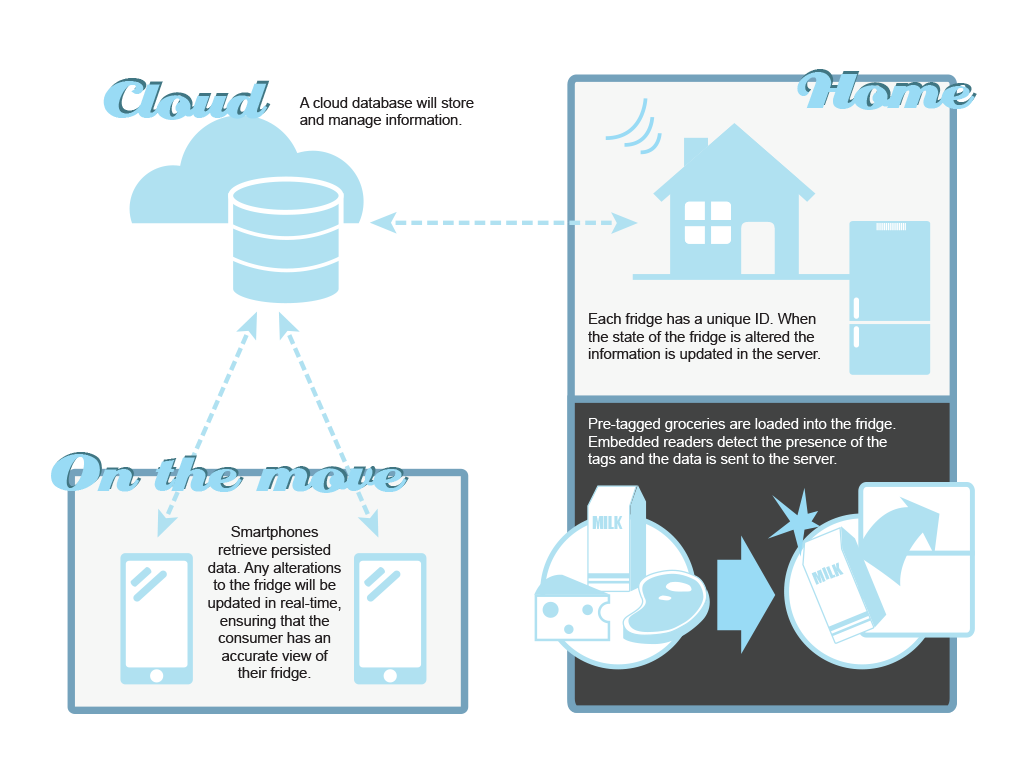
\includegraphics[width=0.85\textwidth]{system2.png}
      \caption{Concept}
\end{figure}

\paragraph{Concept}The proposed concept will incorporate RFID technology as a replacement for barcodes. Groceries will be tagged and granular item-level detail such as use-by-dates, allergy and nutrition information will be accessible through a Smartphone. There will be no need to alter the consumers?  usual behaviour and process of restocking their fridge. Items simply need to be placed in the fridge as usual and the readers will recognise the items as illustrated in figure 1. Any changes in the state of the fridge will be recorded keeping the consumer up to date with their current inventory. Data will be stored using a cloud database giving plenty of leeway for future expansion and highly scalable data retrieval and persistence mechanisms. The information captured will be organised, analysed and presented to the consumer in a user-friendly format via a graphical user interface (GUI). By equipping the consumer with an app over purchasing can be avoided and consumers are reminded to use food before they perish, thus minimising waste. The following features will provide solutions and articulate how the app intends to overcome the issues discovered and discussed in part one.

\vspace{\baselineskip}

\begin{itemize}
  \item Instant look-up of the content of the fridge when away from the home. This feature is intended to dissuade excessive purchasing of groceries and to aid the consumer to make better judgements when faced with detrimental promotional offers from supermarkets.
  
  \item Real-time state monitoring and logging of items. In a scenario where the home has multiple inhabitants the state of the fridge can be altered without all members being aware. The system will keep all inhabitants informed when items are added or removed, avoiding duplicate purchasing and monetary waste.
  
  \item Tracking of itemised inventory, ordered in accordance to the use-by-date. Eliminating the need for consumers to rely on memory alone to memorise when certain products must be used.
  
  \item Statistics analysis of money they have thrown away in the context of food waste can provide motivation for the user to consume purchased foods. Encouraging the minimisation of wastage.
   
   \item Automated meal planning feature using the contents of the fridge alleviating the time consuming process of co-ordinating meals to aid fast pasted lives.
    
   \item Helpful hints such as cooking and freezing to extend the longevity of food. 
   
   \item Recommendation for recipes depending on current inventory to inspire the consumer to create suggested dishes and use the food previously obtained. 

   \item Optimal stocking advice in the form of a shopping list, relative to the number of inhabitants to eliminate over purchasing. 
\end{itemize}

To further clarify the functionality of the app a hypothetical scenario is provided to evoke a vision of how the software will aid the domestic environment. 

\paragraph{Scenario}On the way home from work Rachel visits the supermarket. She consults her smartphone for a reminder of what her fridge contains back at home. A shopping list has been generated for her. She will need less food than the previous week as she has a family dinner scheduled at her mother's this weekend. She browses the poultry aisle and notices a special offer on chicken, `Buy two get the third free' the label reads. According to the application the fridge already contains chicken that must be consumed by tomorrow. She decides against the purchase and carries on, the next item on the list is milk. But then her phone notifies her that her husband Frank has just stocked the fridge with a one litre carton of semi-skimmed milk. She completes the shopping and arrives home to restocks the fridge. Her daughter Ingrid is on the way home from college. Her parents are working late and she must prepare dinner for herself and her younger brother Dean this evening. As she scrolls through the items on the screen of the Smartphone the app recommends cheese and onion quiche. Ready in twenty minutes and one of Dean's favourites. After dinner Ingrid decides to prepare desert, as she unloads the cheesecake from the fridge her Smartphone signals a warning that the cheesecake contains gelatine. Ingrid is a vegetarian, she opts for the yoghurt instead and serves the cheesecake to her brother. At the end of the week a visual chart representing the analysis of the families savings and quantity of food consumed is broadcasted to all the members. They have made a total of \pounds58 savings compared to the previous month. 

\paragraph{Further Extension\dots} This concept can be expanded to other food storage locations such as the pantry or freezer. As more objects become live and the network expands, systems become increasingly sophisticated. Popular wearable devices such as fitness trackers that calculate the amount of calories exhausted can work cooperatively with the home inventory management system and recommend the optimal diet for the individual to lead a healthy lifestyle. Smart shopping solutions such as MyGROCER\cite{myGrocer} could responsibly source personalised promotions sent directly to the consumer via the app.

\vspace{\baselineskip}
\vspace{\baselineskip}
\vspace{\baselineskip}

\subsection{Limitations}

\paragraph{Infrastructure}Although the technology is available the primary set back is the lack of infrastructure in place to support RFID labeled grocery products. It would require significant changes to the supply chain and business processes \cite{pervasiveComp} as experienced by MyGROCER. Barcode printing has it's roots firmly planted in the supply chain and the transition is lagging. With this restriction the prototype will be setup in a hypothetical environment. Central database with sample item details will be made accessible. 

\paragraph{Cost and Environment}Food is mass produced daily resulting in large scale utilisation of tags, this raises concerns for the environment as tags contain non-biodegradable materials such as metal, plastic and petrochemical based materials.\cite{bioTags} Research and production of biodegradable RFID tags are progressing but at the present time it is not available. In the past cost has also effected the move to RFID usage for groceries. The cost of tags has significantly decreased over the past decade but the process of grocery tagging in the supply chain workflow would still require new machinery and alteration to current operations. 

\paragraph{Privacy}Data persistence is a fundamental part of any information system. As computers advance the concerns over privacy has become a controversial topic. At some point, for some length, data must be stored giving opportunities for unethical practices that can lead to the abuse and exploitations of an individual. This seems to be a double-edged sword as when data is used in a responsible and respectful manner it is able to provide people with great advancements to their lives but on the other side, ramification of bad practices can be disruptive and invasive. This bottleneck of obtaining data hinders a system's ability to recommend and persuade meaning the system is only as intelligent as the user allows it to be.
\clearpage

\subsection{Objectives}
The objectives have been stated with consideration given to the time allocated to complete the project. The primary deliverable will take the form of a simple proof of concept to be further developed at a later date. 

\begin{enumerate}

   \item \textbf{Obtain Knowledge of RFID classifications and Reader capabilities}
   	\begin{flushleft}Investigating various classifications of RFID tags and readers to better understand the capabilities and limitation. Based on acquired knowledge, one should gain the expertise to critically assess and select the most appropriate hardware for the use-case of the project.
  	\end{flushleft}
	
   \item \textbf{Tag and Reader Prototype Setup}
   	\begin{flushleft}Achieving an understanding of the underpinnings of RFID technology and tag to reader communications. Successful hardware configuration for demonstration purposes.
  	\end{flushleft}
  
   \item \textbf{Front End Development}
   	\begin{flushleft}Front end development of a simple graphical user interface with minimal functionality, using the Android software development kit (SDK) that will engage with the user. User will view an list of their current inventory.
		  \end{flushleft}
  
   \item \textbf{Back End Configuration of Third-Party Cloud Service}
   	\begin{flushleft}
	Backend configuration using cloud service and exploring cloud service API's. Gain experience of using third-party software, API's and methods of integration. Managing responses from the client side. 
	 \end{flushleft}
	 
	 %Architechted, composition 
	    \item \textbf{Front end, back end Integration}
   	\begin{flushleft}Understanding the RFID stack and the composition of the varying elementes. Managing compatibility issues and adapting to potential change. 
  	\end{flushleft}
 
  \item \textbf{Testing}
   	\begin{flushleft}Delivery of maintainable and transferable code. Gaining confidence and understanding of best practices for production code development. Manual testing using a simple graphical user interface to support the demonstration.
 	\end{flushleft}
 
 \item \textbf{Product Demonstration}
 	\begin{flushleft}Demonstrative prototype and critical evaluation of prototype. Including discussion of application functionality, discoveries and constraints encountered.
 	\end{flushleft}
\end{enumerate}
\clearpage







%........................
% Methodology
%........................
\section{Methodology}

\subsection{System Overview \& Communication Paths}

To better understand the development process figure 2 depicts a simplified system overview and directed communication paths represent the flow of information. Using the client server paradigm the client side application will communicate using the RESTful. The gateway device represents the RFID reader. For this project an Android device with an integrated reader will be utilised. At the middle, AWS will operate. Cloud services are designated the task of persisting and processing data, in addition to the management of the main logic and application deployment. 

\begin{figure}[h!]
  \centering
    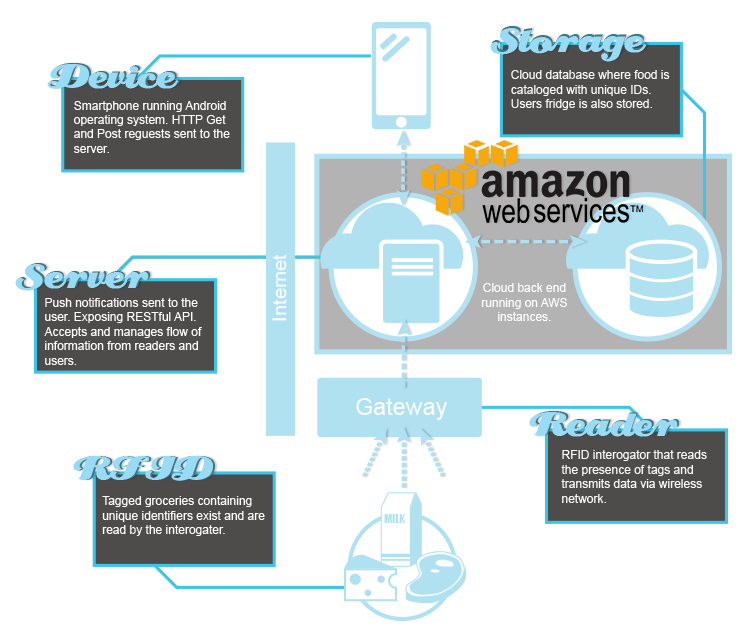
\includegraphics[width=0.85\textwidth]{system6.png}
      \caption{High-Level System Overview.}
\end{figure}

  \vspace{\baselineskip}

\paragraph{Agile}With the heavy use of new and complex technologies the favourable methodology is the agile development methodology. Incremental sprints offer quick prototype generation for fast feedback. This process responds well to change and unpredictable development processes. With the project being an individual effort a pure form of agile is not possible but efforts will be made to follow the methodology closely. At the start of each day objectives and targets will be established for each sprint. Deliverables will be stated in response to previous sprints and necessary changes updated.

\subsection{Development}
Below are stages of development with primary deliverables in correspondence to the objectives in the previous section.

\begin{enumerate}
%1
    \item \textbf{Select RFID \& Label Groceries}
   	\begin{flushleft}Firstly, research on currently available RFID tags will be carried out to understand the limitations and capabilities that will influence the final choice. Cost, range and compatibility will be taken into consideration when selecting a appropriate tag for the use-case. Secondly, investigations of existing systems using RFID to further understand the technology. 
	
	\emph{\textbf{Outcome:}} Selection and application of appropriate tags, together will explanation and backup of the decision. Followed by the discussion of potential performance pay-offs and enhancements that may have influenced the final choice.
	  	\end{flushleft}
	  \vspace{\baselineskip}

   \item \textbf{Research RFID stack}
%2
   	\begin{flushleft}Research the RFID stack and the considerations needed to support interoperability of the system. Understanding the core responsibility of the layers that comprise the stack, leading to the discovery of potential risks and difficulties that may lie ahead.
	
	\emph{\textbf{Outcome:}}Awareness of the various layers of the stack. System design and architecture established and depicted in the form of a visual diagram. Flow charts and activity diagrams created to understand the system processes. 
	\end{flushleft}
	  \vspace{\baselineskip}
%3
   \item \textbf{Setting up the development environment}
   	\begin{flushleft}Installation of integrated development environment (IDE), software development kit (SDK), importing libraries and plugins. RFID enabled Android phone to be used as the reader and a testing platform.  
		
		\emph{\textbf{Outcome:}}  Setup of an environment fit to begin development.
		\end{flushleft}
	  \vspace{\baselineskip}
%4
	   \item \textbf{Tag to reader communication}
   	\begin{flushleft}Use Android SDK's RFID library and implement a simple program that is able to read an RFID tag.
		
	\emph{\textbf{Outcome:}}Simple program that is able to acknowledge the existence of an RFID tag. 
		  \vspace{\baselineskip}

%5
  	\end{flushleft}
	   \item \textbf{Front end development with Android}
   	\begin{flushleft}Using Android SDK develop a client application to manage reader to tag communications through a simple GUI. Java will be the chosen language as supported by the SDK.
	
	\emph{\textbf{Outcome:}} A Java interface and implementation using the RESTful API. A simple GUI to support functionality of client to server communications. 
	\end{flushleft}
	\vspace{\baselineskip}
 
%6
   \item \textbf{Back end Configuration }
   	\begin{flushleft}Backend development using AWS' mobile development SDK. Using Amazon's Lambda API, client messages will be managed. Main logic of the application implemented.
	
	\emph{\textbf{Outcome:}} Program will log the contents of the fridge and the client will be updated when the state of the fridge is altered. Priority listing of items viewable through the GUI.  
	\vspace{\baselineskip}
  	\end{flushleft}
%7
	   \item \textbf{Cloud Database Integration}
   	\begin{flushleft} Configure Amazon's DynamoDB to respond to server requests. Create a central database for global product information to be stored.
	
	\emph{\textbf{Outcome:}} Central database containing a few items for demonstration purposes created for the storage of item details. 
	\vspace{\baselineskip}
  	\end{flushleft}
	 
%8	
   \item \textbf{Testing}
   	\begin{flushleft}Tests will be carried out and documented throughout the process. Upon reflection of past implementation, current situation will be influenced. Unit tests and mocking frame works may be used to support best practices where appropriate.
	  	
	\emph{\textbf{Outcome:}} Manual test and documentation of test results and critical analysis of each stage. Sufficient unit test coverage for code.
	\vspace{\baselineskip}
  	\end{flushleft}
%9	
	   \item \textbf{Demonstration}
   	\begin{flushleft}Creating demonstration of application functionality of the prototype and critically assess the product. Reflect on the development process and discuss leaning outcomes. 
	
	\emph{\textbf{Outcome:}}A proof of concept with simple functionality in the form of an Android application.
	  	\end{flushleft}
\end{enumerate}
\vspace{\baselineskip}


\vspace{\baselineskip}
\vspace{\baselineskip}
\vspace{\baselineskip}

\subsection{Risks \& Pitfalls}
\paragraph{New Technology}When attempting to build new systems there is a high possibility of encountering unexpected problems. Solving of the issue could slow the development process and originally planned schedules may be forced to change. 

\paragraph{Architecture}The design decision regarding system architecture. Balancing system performance to payoff and making the correct choice under pressure of limited time. The wrong choice may result in high latency or incompatible components.   

\paragraph{Compatibility}The compatibility of components is crucial. Using unfamiliar technologies there is always a likelihood of incompatibilities that could cause production difficulties that interrupt the development process. 

\paragraph{Languages}The integration of components usually require the use of multiple programming languages causing unpredictable learning curves that could halt development. 

\clearpage

%........................
% Schedule
%........................


\section{Schedule}

%\begin{preview}
\tikzset{every picture/.style={xscale=0.85,transform shape}}
  \begin{gantt}{10}{12}
    \begin{ganttitle}
    \numtitle{1}{1}{12}{1}
    \end{ganttitle}
    \ganttbar[color=cyan]{1}{0}{1}
    \ganttbar[color=cyan]{2}{1}{1}
    \ganttbar[color=cyan]{3}{2}{0.5}
     \ganttbar[color=cyan]{4}{2.5}{1.5}
   % \ganttmilestone[color=cyan]{3}{4}
    \ganttbar[color=cyan]{5}{4}{2}{10}
    \ganttbar[color=cyan]{6}{6}{2}
    \ganttbar[color=cyan]{7}{8}{2}
    \ganttbar[color=cyan]{8}{4}{6}{5}
    %\ganttcon{4}{5}{4}{6}
    %\ganttmilestonecon{8}{6}
    \ganttbar[color=cyan]{9}{10}{2}{5}
  \end{gantt}
  
%\end{preview}

\subsection{Timetable}

The above gantt chart represents the schedule for the project commencing form the 22nd June 2015 to the 14 September 2015. The horizontal numbers represent the number of weeks available to complete the project and the vertical digits corresponds to the stages of development mentioned in the previous section. As the agile methodology is used diversion form the plan is anticipated. Continuous testing will occur throughout the development process. The final two weeks will be allocated for the documentation in the form of a report. 

\vspace{\baselineskip}

\begin{enumerate}
	\item RFID Research and documentation of findings.
	\item RFID Stack Research
	\item Environment Setup
	\item Tag to Reader Communication
	\item Front End Development
	\item Back End Development
	\item Database Configuratiion
	\item Testing
	\item Report detailing and final review of project in preparation for submission and report.
 \end{enumerate}

\iffalse
\paragraph{\textbf{Week 1: 8th June:	}} \textbf{\emph{Development stage 1:}}
\begin{itemize}
  \item  RFID Research and documentation of findings.
\end{itemize}

\paragraph{\textbf{Week 2: 15th June:}} \textbf{\emph{Development stage 2: }}
\begin{itemize}
  \item RFID stack and system design research.
  \item Document discoveries.
  \item Create system diagram. 
\end{itemize}

\paragraph{\textbf{Week 3: 22th June:}}  \textbf{\emph{Development stage 3-4: }}
\begin{itemize}
  \item Development environment setup. 
  \item Begin research of Android mobile development. 
\end{itemize}

\paragraph{\textbf{Week 4: 29th June:}}  \textbf{\emph{Development stage 4: }}
\begin{itemize}
  \item Reader to recognise tag
  \end{itemize}
\paragraph{\textbf{Week 5-7: 6th July-27th July:}} \textbf{\emph{Development stage 5: }}


%\paragraph{\textbf{Week 6: 13th July:	}} \textbf{\emph{Development stage 5: }}

%\paragraph{\textbf{Week 7: 20th July:	}} \textbf{\emph{Development stage 5: }}

\paragraph{\textbf{Week 7-10: 27th July-17th August:}} \textbf{\emph{Development stage 6: }}

%\paragraph{\textbf{Week 9: 3th August:	}} \textbf{\emph{Development stage 6: }}

%\paragraph{\textbf{Week 10: 10th August:	}} \textbf{\emph{Development stage 6: }}

\paragraph{\textbf{Week 11: 17th August-24th August:	}} \textbf{\emph{Development stage 6: }}

\paragraph{\textbf{Week 12: 24th August:	}} \textbf{\emph{Development stage 7: }}

\paragraph{\textbf{Week 13: 31th August:	}} \textbf{\emph{Development stage 7: }}

\paragraph{\textbf{Week 14: 7th September:	}} \textbf{\emph{Development stage 9: }}

\paragraph{\textbf{Week 15: 14th September:	}} 

\fi
\clearpage
%........................
% Bibliography
%........................


% [5] U. J. Gelinas, et al., Business Processes and Information Technology. Cincinnati: South-Western/%Thomson Learning, 2004.
\begin{thebibliography}{29}

\bibitem{waste}W. Carr, E.Downing, \emph{\say{Food Waste}}, Science and Environment Section, House of Commons, 2 December 2014
\vspace{\baselineskip}

\bibitem{FoodWaste}European Union Committee, \emph{\say{Counting the Cost of Food Waste: EU Food Waste Prevention}}, London : The Stationery Office Limited, House of Lords, 6 April 2014
\vspace{\baselineskip}

\bibitem{memory}G.A Miller, \emph{\say{Magical Number Seven, Plus or Minus Two: Some Limits on Our Capacity for Processing Information}}, vol. 63. Cambridge, MA: The Psychological Review, 1956.
\vspace{\baselineskip}

\bibitem{WRAP}P.Whitehead \emph{et al}, \emph{\say{Estimates of waste in the food and drink supply chain}}, WRAP, July 2002.
\vspace{\baselineskip}

\bibitem{obesity}M. White, \emph{\say{Food access and obesity.}} Obesity reviews 8.s1 (2007): 99-107.
\vspace{\baselineskip}

\bibitem{statistic}Government Statistical Service, \emph{\say{Uk Statistics on waste 2010-2012}}, Department for Environment, food and Rural Affairs, March 2015
\vspace{\baselineskip}

\bibitem{idiotFridge}Susie Steiner, \emph{\say{Smart fridge? Idiot fridge, more like}}, The Guardian, January 11th 2014
\vspace{\baselineskip}

\bibitem{motivation}Graham-Rowe, Ella, Donna C. Jessop, and Paul Sparks.\emph{\say{Identifying motivations and barriers to minimising household food waste.}} Resources, Conservation and Recycling 84 (2014): 15-23.
\vspace{\baselineskip}

\bibitem{horsy}Environment, Food and Rural Affairs Committee, \emph{\say{Food Contamination}},vol. 1, authority of the House of Commons London: The Stationery Office Limited, 2013.
\vspace{\baselineskip}

\bibitem{anarobic}Li, Lei, \emph{et al.} \emph{\say{Early warning indicators for monitoring the process failure of anaerobic digestion system of food waste.}} Bioresource technology 171 (2014): 491-494.
\vspace{\baselineskip}

\bibitem{nano}Handford, Caroline E., et al, \emph{\say{Implications of nanotechnology for the agri-food industry: Opportunities, benefits and risks}}, Trends in Food Science \& Technology 40.2 2014: 226-241.
\vspace{\baselineskip}

\bibitem{georgeR}G. Roussos, \emph{\say{Networked RFID System, software \& services}}, 1st edition, Springer, August 29, 2008
\vspace{\baselineskip}

\bibitem{rfidFood} R. Chen, \emph{\say{Using RFID Technology in Food Produce Traceability}},WSEAS Transaction on information science and applications, November 2008
\vspace{\baselineskip}

\bibitem{rfidFood2}S. Piramuthu, \emph{et al.}, \emph{\say{RFID-generated traceability for contaminated product recall in perishable food supply networks.}} European Journal of Operational Research 225.2 (2013): 253-262.?\vspace{\baselineskip}

\bibitem{coke}T. Lane, \emph{\say{"The Only Coke Machine on the Internet"}}, Carnegie-Mellon CS department, 1990
\vspace{\baselineskip}

\bibitem{retailRFID}G. Roussos, \emph{\say{Enabling RFID in Retail}}, IEEE Computer Society, 2006
\vspace{\baselineskip}

\bibitem{RFID}A. Sabbaghi, G. Vaidyanathan, \emph{\say{Effectiveness and Efficiency of RFID technology in Supply Chain Management: Strategic values and Challenges}}, Journal of Theoretical and Applied Electronic Commerce Research, April 2008

\bibitem{FSA}Food Standard Agency, \emph{\say{Country of Origin Labelling Guidance}}, October 2008
\vspace{\baselineskip}

\bibitem{FDA}FDA, \emph{\say{Sweet Sam's Baking Company Issues Allergy Alert on Undeclared Milk in Starbucks Black \& White Mini Cookies}}, Firm Press Release, April 13th 2015

\bibitem{fukushima}World Health Organisation, \emph{\say{Health risk assessment from the nuclear accident after the 2011 Great East Japan Earthquake and Tsunami based on a preliminary dose estimation}}, ISBN9789241505130 Geneva, Switzerland: WHO Press, 2013
\vspace{\baselineskip}

\bibitem{myGrocer}P. Kourouthanasis\emph{et al.}, \emph{\say{Intelligent cokes and diapers: MyGrocer ubiquitous computing environment}}, First International Mobile Business Conference, pp. 150--172, July 2002.
\vspace{\baselineskip}

\bibitem{weiser}M. Weiser, \emph{\say{Creating the invisible interface}}, 7th annual ACM symposium on User interface software and technology, 1994
\vspace{\baselineskip}

\bibitem{weiserLimit}M. Weiser, \emph{\say{Some Computer Science Issues in Ubiquitous Computing}}, CACM, July 1993
\vspace{\baselineskip}

\bibitem{HadoopInAction}C. Lam, \emph{\say{Hadoop in Action}}, 1st edition, Manning Publications, 25th Dec. 2010
\vspace{\baselineskip}

\bibitem{CAYS}J. Rosenberg, \emph{\say{The Cloud t Your Service}}, Manning Publications; 1 edition, 2010
\vspace{\baselineskip}

\bibitem{GS1}?GS1, \emph{\say{RFID Bar Code Interoperability GS1 Guideline}}, GS1 Global Office, August 10th 2012
\vspace{\baselineskip}

\bibitem{pervasiveComp}P. Kourouthanassis, G. Roussos, \emph{\say{Developing Consumer- Friendly Pervasive Retail Systems}}, IEEE, Page(s): 32	- 39, 2003
\vspace{\baselineskip}

\bibitem{bioTags}Y. Duroc, D. Kaddour, \emph{\say{RFID potential impacts and future evolution for green projects}},26000 Valence, France, Elsevier Ltd, 2012
\vspace{\baselineskip}

\end{thebibliography}

\end{document}
\setlength{\parindent}{0pt}
\begin{document}


\end{document}
